%%=============================================================================
%% Methodologie
%%=============================================================================

\chapter{\IfLanguageName{dutch}{Methodologie}{Methodology}}
\label{ch:methodologie}

%% TODO: Hoe ben je te werk gegaan? Verdeel je onderzoek in grote fasen, en
%% licht in elke fase toe welke stappen je gevolgd hebt. Verantwoord waarom je
%% op deze manier te werk gegaan bent. Je moet kunnen aantonen dat je de best
%% mogelijke manier toegepast hebt om een antwoord te vinden op de
%% onderzoeksvraag.

%TODO korte inleiding tot hoofdstuk

\section{Opstellen use cases}
\label{sec:opstellen-use-cases}

Huis van Alijn heeft een grote fotocollectie over het dagelijkse leven in Belgi\"{e} in de 20\textsuperscript{e} en 21\textsuperscript{e} eeuw. Dit zijn foto’s die ontvangen werden via schenkingen of die gekocht werden op rommelmarkten. Vaak is er amper contextuele informatie en is er niet geweten wie of wat op de foto staat. 

Om de foto’s te kunnen ontsluiten of te doorzoeken, heeft het museum nood aan metadata die een idee geven van wat er op het beeld staat. Uit een gesprek met Astrid Vergauwe, digitaal strateeg van Huis van Alijn en Industriemuseum, bleek dat het museum de foto’s indeelt in een aantal thema’s (bv. \textit{huwelijk}, \textit{vakantie} en \textit{speelgoed}) en in het decennium waarin de foto’s getrokken worden (bv. 50s, 60s). Het zou voor het museum een enorme hulp zijn als via beeldherkenning de beelden voorzien worden van beschrijvende metadata en ingedeeld worden in de thema’s en periodes.

Aan Huis van Alijn werd voorgesteld om volgende use cases te onderzoeken:
\begin{itemize}
	\item het automatisch metadateren van iedere foto door het ingebouwde model van de CV API.
	\item het classificeren van de foto’s in de thema’s die door Huis van Alijn voorgesteld worden. Hiervoor wordt een \textit{custom} model gecre\"{e}erd en wordt de CV API getraind. We gaan ook na of het mogelijk is om die classificatie te doen op basis van de tags uit het ingebouwde model van de CV API. Vermoedelijk zal het slagen hiervan afhangen van hoe vertrouwd het model met het thema is. 
	\item het indelen van de foto’s in de decennia waarin ze gemaakt werden. Ook hiervoor wordt een custom model ontwikkeld en wordt de CV API getraind.
\end{itemize}

\section{Analyseren van de dataset}
\label{sec:analyseren-van-de-dataset}

Het Huis van Alijn leverde een set van 845 beelden aan uit de \textit{Anonieme snapshots} collectie die bestaat uit vijf thema’s en tien decennia. Alle beelden hadden reeds metadata zodat de tags van de CV API vergeleken kon worden met de bestaande beschrijvingen. In tabel  \ref{tab:analyse-dataset} wordt de spreiding van de foto’s per thema en periode getoond.

\begin{table}
	\centering
	\begin{tabular}{l|ccccc|r}
		\toprule
		& Geboorte & Huwelijk & Sint & Speelgoed & Vakantie & Totaal \\
		\midrule
		00s & 6 & 1 & 0 &2 & 0 & \textbf{9} \\
		10s & 10 & 4 & 0 & 2 & 0 & \textbf{16} \\
		20s & 4 & 13 & 0 & 4 & 11 & \textbf{32} \\
		30s & 2 & 20 & 0 & 10 & 22 & \textbf{54} \\
		40s & 6 & 26 & 13 & 16 & 0 & \textbf{61} \\
		50s & 15 & 82 & 82 & 14 & 16 & \textbf{209} \\
		60s & 18 & 169 & 0 & 11 & 28 & \textbf{226} \\
		70s & 21 & 55 & 2 & 19 & 17 & \textbf{114} \\
		80s & 11 & 14 & 0 & 17 & 19 & \textbf{61} \\
		90s & 3 & 9 & 0 & 6 & 3 & \textbf{21} \\
		onbekend & 0 & 7 & 0 & 0 & 35 & \textbf{42} \\
		\midrule
		\textbf{Totaal} & \textbf{96} & \textbf{400} & \textbf{97} & \textbf{101} & \textbf{151} & \textbf{845} \\
		\bottomrule
	\end{tabular}
	\caption[opdeling van de foto’s per thema en decennia]{De opdeling van de foto’s per thema (kolommen) en per decennia (rijen). De gekleurde cellen duiden op een overgewicht van de foto’s per thema of periode}
	\label{tab:analyse-dataset}
\end{table}

%TODO denk aan grafieken om de ongelijke verdeling van de dataset te duiden
Het valt hierbij op dat de dataset ongelijk verdeeld is:
\begin{itemize}
	%TODO denk aan hoofdletters --> opzoeken
	\item bijna de helft van de dataset bestaat uit huwelijksfoto’s. De andere thema’s zijn meer gelijk verdeeld met grofweg honderd foto’s per thema. 
	\item daarenboven concentreren de huwelijksfoto’s zich op drie periodes. Bijna 75\% van de foto’s zijn afkomstig uit de periode 50s, 60s en 70s. 
	\item de Sinterklaasfoto’s zijn afkomstig uit slechts drie periodes (40s, 50s en 70s) waarvan bijna 85\% uit één periode (50s).
	\item de ongelijke verdeling van de foto’s per thema heeft ook een gevolg op de foto’s per periode. Er zijn vooral foto’s afkomstig uit de periodes 50s, 60s en 70s. Voor 50s gaan bijna 80\% van de foto’s over huwelijk en Sinterklaas, voor de 60s bijna 75\% over huwelijk en voor de 70s zijn 50\% huwelijksfoto’s. Van de vroegste periodes (00s en 10s) zijn dan weer weinig foto’s. 
	\item zowel Sinterklaas- als vakantiefoto’s komen niet in alle periodes voor.
\end{itemize}

Bij het interpreteren van de resultaten moet rekening gehouden worden met deze ongelijke verdeling.

\section{Keuze voor API}
\label{sec:keuze-voor-api}

Clarifai werd als API gekozen om de onderzoeksvraag te beantwoorden. 

Clarifai is gesticht in 2013 door Matthew Zeiler. Hij had in 2013 deelgenomen aan de ImageNet Challenge als doctoraatsstudent samen met zijn promotor Dr. Rob Fergus. Hun architectuur, ZFNet, waarop ook Clarifai gebouwd is, was de winnaar van de ImageNet Challenge~\autocite{Tsang2018}.

De keuze viel op deze API om een aantal redenen:
\begin{enumerate}
	\item De website bevat goede en duidelijke documentatie om met de API aan de slag te gaan. De uitleg wordt telkens voorzien van een voorbeeld in de ondersteunde programmeertalen. %TODO link naar documentatie
	\item De API heeft clients in verschillende programmeertalen die het de ontwikkelaar mogelijk maken om de API te gebruiken in de programmeertaal naar keuze. JavaScript, Python, Java, C\# en PHP hebben officiële clients die door Clarifai ondersteund en ontwikkeld worden. De REST API kan ook rechtstreeks bevraagd worden zonder gebruikt van een API client.
	\item De Clarifai website beschikt over een grafische interface waarin gebruikers beelden kunnen opladen om ze te laten taggen door een van de ingebouwde modellen of een nieuw model kunnen trainen. Dit verhoogt het gebruiksgemak, wat, zoals besproken in~\ref{sec:probleemstelling}, een belangrijke factor was bij de keuze voor een API.
	\item Er zijn verschillende ingebouwde modellen die gebruikt kunnen worden om beelden te taggen, gaande van zeer algemene modellen (het general model) tot zeer specifieke modellen, zoals een model om modeconcepten te herkennen of een model om elementen met betrekking tot voeding en vaatwerk te detecteren.
\end{enumerate}

\section{Beelden beschikbaar maken via een publieke URL}

%TODO uitleggen waarom geen base64
Het Huis van Alijn bracht ons de beelden aan op een harde schijf. De beelden waren immers nog niet online beschikbaar. Om op een geautomatiseerde manier de API van Clarifai te kunnen bevragen, moest een publieke URL voor de beelden voorzien worden. Het waren hoge resolutie beelden waarvan het merendeel in TIFF-formaat was en een kleiner deel in JPEG-formaat. De meeste beelden hadden daarom een bestandsgrootte (10 \'{a} 13 MB per beeld) die te groot is voor Clarifai. Clarifai wil immers beelden met een grootte van maximum 3,6 MB. 

De beelden werden daarom op een beeldenserver geplaatst waarmee met een URL het beeld opgevraagd kon worden in een kleinere bestandsgrootte in het JPEG-bestandsformaat. Clarifai kan immers niet omgaan met beelden groter dan 3,6 MB. Een andere optie was om de beelden te converteren naar JPEG, ze daarbij te verkleinen naar een breedte van 512 pixels en ze vervolgens op een webserver of FTP-server te plaatsen. Clarifai verkleint immers zelf alle beelden tot 512 pixels en hoe dichter je bij dat formaat komt, hoe sneller de API calls verlopen~\autocite{Clairbot2019}. Dit laatste ontdekten we echter pas nadat de test al uitgevoerd was. Het was namelijk niet opgenomen in de documentatie.

De beelden werden opgeladen in een Amazon AWS EC2 Ubuntu instance waarop de beeldenserver (Cantaloupe) ge\"{i}nstalleerd was. Op die manier kreeg ieder beeld een publieke URL die gebruikt kon worden bij het aanroepen van de Clarifai API.

\section{Beschikbare metadata verzamelen in een CSV}
\label{sec:metadata-verzamelen-csv}

De 845 beelden van Huis van Alijn waren voorzien van metadata die uit de bestandsnaam van de digitale bestanden gehaald konden worden. De bestandsnamen hadden volgende logica waarmee het oorspronkelijke medium van het digitale bestand (foto of dia) en het decennium waarin de foto gemaakt was, gehaald kon worden: MEDIUM-DECENNIUM-VOLGNUMMER. Bestanden die startten met \textit{FO} waren digitale kopieën van foto’s, zij die startten met \textit{DIA} van diapositieven. 

Er werd een CSV gecreëerd waarin alle beschikbare metadata per beeld verzameld werden:
\begin{itemize}
	\item base (URL): de URL van het beeld die in vorige stap gecreëerd werd;
	\item bestandsnaam of ID van het beeld;
	\item de extensie of het oorspronkelijke bestandsformaat van het beeld: .tif of .jpg;
	\item type: foto, diapositief of onbekend;
	\item thema;
	\item periode (decennium)
\end{itemize}

%TODO voetnoot toevoegen
Om deze informatie te verzamelen, werd een shell script geschreven. Op de harde schijf waren de afbeeldingen verzameld in een mapje (directory) per thema. Informatie zoals extensie, type, thema en periode werden uit de bestandsnaam gehaald. 

\section{Uitvoeren van workflows}
\label{sec:uitvoeren-workflows}

Er werden twee workflows een aantal keer doorlopen bij het uitvoeren van dit onderzoek:
\begin{itemize}
	\item een workflow om de beelden te laten taggen door Clarifai;
	\item een workflow om via training een custom model te cre\"{e}ren.
\end{itemize}

\subsection{Workflow 1: Een dataset laten taggen door Clarifai}
\label{subsec:workflow1}

%TODO nadenken of van de onderstaande twee subsubsections geen subsection gemaakt kan worden.
\subsubsection{De Clarifai API aanroepen}

Clarifai beschikt over API-clients in verschillende programmeertalen (Java, Python, Javascript, C\#, Objective-C en PHP), maar doordat we zelf het meeste voeling hebben met shell scripting, werd gekozen om de REST API te bevragen via cURL, een command-line programma voor het verkrijgen of verzenden van bestanden met behulp van  een URL.

Een API key is nodig om de API te bevragen. Daarom werd eerst een account bij Clarifai aangemaakt. Automatisch verkrijg je dan een gratis key. 

%TODO screenshot van aanmaken van account

Het general model van Clarifai werd gebruikt om de volledige dataset van Huis van Alijn te taggen. Dit is namelijk het meest uitgebreide model met de meeste concepten. het bevat ongeveer 11.000 verschillende concepten waaronder objecten, thema's, emoties in verschillende talen. Daardoor kan het model gebruikt worden voor een reeks van zeer uiteenlopende beelden.{ClarifaiGeneral}

Om via de Clarifai API tags te krijgen voor een beeldbestand via het general model, moet onderstaande commando ingegeven worden in de command line. \$\{API\_key\} en \$\{url\_naar\_het\_beeld\} moeten vervangen worden door respectievelijk de API key en de URL van het beeld~\autocite{ClarifaiAPI}.

%TODO toevoegen van model_id en version_id

\begin{lstlisting}[language=bash,caption=bash commando om een beeld door Clarifai te laten taggen.]
#!/bin/bash
curl -X POST
    -H 'Authorization: Key "${API_key}"'
    -H 'Content-Type: application/json'
    -d '{
        "inputs": [{
            "data": {
                "image": { 
                    "url": "${url_naar_het_beeld}"
                    }
                }
            }
        ]
    }'
"https://api.clarifai.com/v2/models/${model_id}/versions/${version_id}/outputs"
\end{lstlisting}

Om de API te bevragen, werd een shell script geschreven.\footnote{\url{https://github.com/nvanderperren/bachelorproef/blob/master/research/scripts/predict_image.sh})} Het bevragen van de API verliep vlot. Gemiddeld waren er per beeld twee à drie seconden nodig. Bij drie beelden mislukte het aanroepen omdat ze een te groot bestandsgrootte hadden. Deze beelden werden verkleind waarna de API opnieuw aangeroepen werd.\footnote{voor deze beelden werd een nieuw script geschreven waarin de gewenste grootte en de bestandsnaam van de beelden als parameter meegegeven kan worden: \url{https://github.com/nvanderperren/bachelorproef/blob/master/research/scripts/predict_image_by_size_id.sh}. Er werd gekozen om alles zoveel mogelijk in een script te zetten in functie van hergebruik.}

\subsubsection{Tags van API in een overzicht verzamelen}

Na het bevragen van de Clarifai API werd per beeld een API response in JSON ontvangen met daarin onder meer de tags die aan de beelden gegeven werden.

\begin{lstlisting}[language=json,caption=een ingekorte versie van een ontvangen API response met voorspellingen van Clarifai .]
{
  "status": {
    "code": 10000,
    "description": "Ok",
    "req_id": "7a70efb773234ba9a3eaf219328782b4"
  },
  "outputs": [{
    "id": "94b039d533454d53b01f2d3f825a097e",
    "status": {
      "code": 10000,
      "description": "Ok"
    },
    "created_at": "2019-04-01T16:14:28.886109228Z",
    "model": {
      "id": "aaa03c23b3724a16a56b629203edc62c",
      "name": "general",
      "created_at": "2016-03-09T17:11:39.608845Z",
      "app_id": "main",
      "output_info": {
        "message": "Show output_info with: GET /models/{model_id}/output_info",
        "type": "concept",
        "type_ext": "concept"
      },
      "model_version": {
        "id": "aa7f35c01e0642fda5cf400f543e7c40",
        "created_at": "2018-03-06T21:10:24.454834Z",
        "status": {
       	  "code": 21100,
          "description": "Model trained successfully"
        }
      },
      "display_name": "General"
   	},
    "input": {
      "id": "d74a5f9d8961406eb5a15e9172be9399",
      "data": {
        "image": {
          "url": "http://ec2-18-191-252-182.us-east-2.compute.amazonaws.com:8182/iiif/2/FO-30-00197/full/full/0/default.jpg"
        }
      }
    },
    "data": {
      "concepts": [{
        "id": "ai_l8TKp2h5",
        "name": "people",
        "value": 0.999308,
        "app_id": "main"
      },{
        "id": "ai_bmls4LpL",
        "name": "group",
        "value": 0.9847269,
        "app_id": "main"
      },{
        "id": "ai_sd6DKdXp",
        "name": "group together",
        "value": 0.9833066,
        "app_id": "main"
      },{
        "id": "ai_RQccV41p",
        "name": "woman",
        "value": 0.9795268,
        "app_id": "main"
      },{
        "id": "ai_VPmHr5bm",
        "name": "adult",
        "value": 0.97893196,
        "app_id": "main"
      }]
    }
  }]
}
\end{lstlisting}

De gegevens werden verzameld in een CSV-bestand die geïmporteerd zal worden in Google Sheets. Google Sheets heeft als voordeel dat resultaten eenvoudig gedeeld kunnen worden met de museummedewerkers en bezit bovendien over ingebouwde reken- en queryfuncties die het analyseren van de resultaten vereenvoudigen. Bovendien kan Google Sheets afbeeldingen in een cel tonen via de IMAGE-functie\footnote{Voor meer info, zie: \url{https://support.google.com/docs/answer/3093333?hl=en}}. Dit maakt het veel eenvoudiger om de gegevens te valideren.

Om de tags uit de JSON-bestanden te halen werd een shell script geschreven die per beeld de tags en de waarschijnlijkheidsscore uitleest. Het paste-commando werd vervolgens gebruikt om deze CSV samen te voegen met de CSV uit \textit{\ref{sec:metadata-verzamelen-csv} Beschikbare metadata verzamelen in CSV}.

%TODO opnemen van eerste regels van CSV?

\subsubsection{Gegevens valideren}

Om de kwaliteit van de tags te controleren, werd dezelfde methodologie gebruikt als in \textcite{Vanstappen2019}. In het Google Sheets document werd bij ieder tag een checkbox geplaatst die door de validator aangevinkt moest worden als de tag correct was. Dit had als voordeel dat de validatie relatief snel kon gebeuren en dat ook het verwerken van de resultaten eenvoudig was. 

Tijdens het valideren bleek het aanvinken van correcte tags toch niet zo eenvoudig te zijn. Sommige tags vereisten enige interpretatie die moeilijk is zonder de context van het beeld te kennen. Het gaat om tags zoals \textit{happy}, \textit{music} en \textit{love}. Daarvoor konden we ons baseren op de thema’s van de foto’s. We gingen ervan uit dat mensen op huwelijksfoto’s en geboortefoto’s vol liefde waren, en dat zij, net als mensen op vakantie, gelukkig zijn. 

Een andere moeilijkheid was het herkennen of de kinderen op de foto jongens of meisjes waren, of dat we de mensen op de foto konden beschouwen als bejaarde mensen of niet. We zijn bij het corrigeren van deze tags niet te streng geweest. Bij twijfel, wanneer bijvoorbeeld zowel de tags \textit{boy} als \textit{girl} voorkwamen, hebben we steeds de term met de grootste waarschijnlijkheidsscore goedgekeurd.

Ten slotte waren er ook nog de tags \textit{group}, \textit{several} en \textit{many}. We beschouwden iets een groep als er drie of meer mensen op de foto stonden. De andere tags werden gevoelsmatig goed- of afgekeurd.

\begin{figure}
	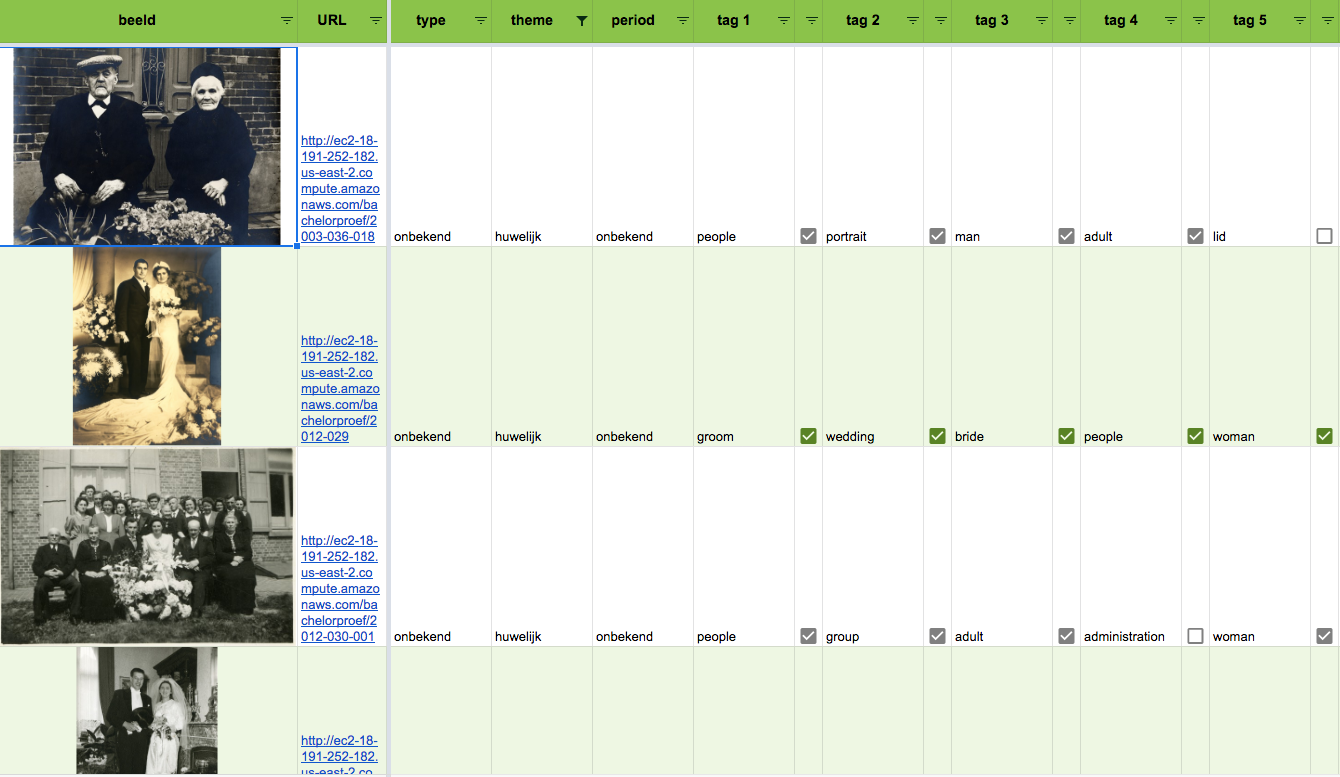
\includegraphics[width=\textwidth]
	{validatiescherm.png}
	\caption{Screenshot van de Google Sheet waarin de validatie plaatsvond.}
	\label{fig:validatiescherm}
\end{figure}

\subsection{Workflow 2: Een custom model trainen}